
\begin{figure}
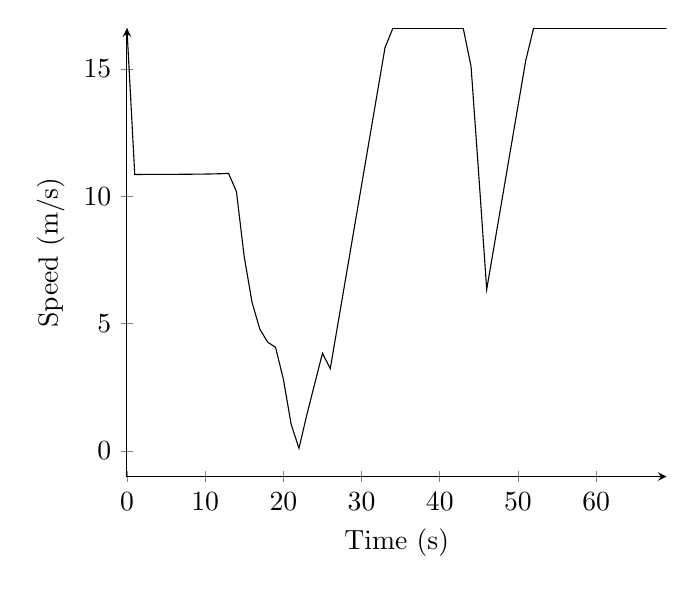
\begin{tikzpicture}
\begin{axis}[
legend style={anchor=west},
axis x line=bottom,
axis y line=left,
ymin=-1,
xlabel=Time (s),
ylabel=Speed (m/s),
]
\addplot[] coordinates {
(0, 16.6)
(1, 10.8589149147)
(2, 10.8596208126)
(3, 10.8604563735)
(4, 10.8614554413)
(5, 10.8626636799)
(6, 10.8641439023)
(7, 10.865984433)
(8, 10.8683126544)
(9, 10.8713177691)
(10, 10.875290729)
(11, 10.8806979419)
(12, 10.8883259874)
(13, 10.8995882858)
(14, 10.1873418808)
(15, 7.62178789854)
(16, 5.83399494698)
(17, 4.7827612542)
(18, 4.27490600835)
(19, 4.0755870069)
(20, 2.82939142039)
(21, 1.04656835382)
(22, 0.108726959206)
(23, 1.42197324749)
(24, 2.63164197623)
(25, 3.83907185999)
(26, 3.23654108147)
(27, 5.03654108147)
(28, 6.83654108147)
(29, 8.63654108147)
(30, 10.4365410815)
(31, 12.2365410815)
(32, 14.0365410815)
(33, 15.8365410815)
(34, 16.6)
(35, 16.6)
(36, 16.6)
(37, 16.6)
(38, 16.6)
(39, 16.6)
(40, 16.6)
(41, 16.6)
(42, 16.6)
(43, 16.6)
(44, 15.1032182119)
(45, 10.7871119847)
(46, 6.34349160366)
(47, 8.14349160366)
(48, 9.94349160366)
(49, 11.7434916037)
(50, 13.5434916037)
(51, 15.3434916037)
(52, 16.6)
(53, 16.6)
(54, 16.6)
(55, 16.6)
(56, 16.6)
(57, 16.6)
(58, 16.6)
(59, 16.6)
(60, 16.6)
(61, 16.6)
(62, 16.6)
(63, 16.6)
(64, 16.6)
(65, 16.6)
(66, 16.6)
(67, 16.6)
(68, 16.6)
(69, 16.6)
};

\end{axis}
\end{tikzpicture}
\label{tik:speed:100:6}
\caption{100 percent diving with GSC on route $6$}
\end{figure}
